%%%%%%%%%%%%%%%%%%%%%%%%%%%%%%%%%%%%%%%%%
% Lachaise Assignment
% LaTeX Template
% Version 1.0 (26/6/2018)
%
% This template originates from:
% http://www.LaTeXTemplates.com
%
% Authors:
% Marion Lachaise & François Févotte
% Vel (vel@LaTeXTemplates.com)
%
% License:
% CC BY-NC-SA 3.0 (http://creativecommons.org/licenses/by-nc-sa/3.0/)
% 
%%%%%%%%%%%%%%%%%%%%%%%%%%%%%%%%%%%%%%%%%

%----------------------------------------------------------------------------------------
%	PACKAGES AND OTHER DOCUMENT CONFIGURATIONS
%----------------------------------------------------------------------------------------

\documentclass{article}

%%%%%%%%%%%%%%%%%%%%%%%%%%%%%%%%%%%%%%%%%
% Lachaise Assignment
% Structure Specification File
% Version 1.0 (26/6/2018)
%
% This template originates from:
% http://www.LaTeXTemplates.com
%
% Authors:
% Marion Lachaise & François Févotte
% Vel (vel@LaTeXTemplates.com)
%
% License:
% CC BY-NC-SA 3.0 (http://creativecommons.org/licenses/by-nc-sa/3.0/)
% 
%%%%%%%%%%%%%%%%%%%%%%%%%%%%%%%%%%%%%%%%%

%------------------------------------------%
% 		PARTE NOSSA 
%------------------------------------------%

\usepackage[portuguese]{babel}	

%----------------------------------------------------------------------------------------
%	PACKAGES AND OTHER DOCUMENT CONFIGURATIONS
%----------------------------------------------------------------------------------------


\usepackage{amsmath,amsfonts,stmaryrd,amssymb} % Math packages

\usepackage{enumerate} % Custom item numbers for enumerations

\usepackage[ruled]{algorithm2e} % Algorithms

\usepackage[framemethod=tikz]{mdframed} % Allows defining custom boxed/framed environments

\usepackage{listings} % File listings, with syntax highlighting
\lstset{
	basicstyle=\ttfamily, % Typeset listings in monospace font
}

%----------------------------------------------------------------------------------------
%	DOCUMENT MARGINS
%----------------------------------------------------------------------------------------

\usepackage{geometry} % Required for adjusting page dimensions and margins

\geometry{
	paper=a4paper, % Paper size, change to letterpaper for US letter size
	top=2.5cm, % Top margin
	bottom=3cm, % Bottom margin
	left=2.5cm, % Left margin
	right=2.5cm, % Right margin
	headheight=14pt, % Header height
	footskip=1.5cm, % Space from the bottom margin to the baseline of the footer
	headsep=1.2cm, % Space from the top margin to the baseline of the header
	%showframe, % Uncomment to show how the type block is set on the page
}

%----------------------------------------------------------------------------------------
%	FONTS
%----------------------------------------------------------------------------------------

\usepackage[utf8]{inputenc} % Required for inputting international characters
\usepackage[T1]{fontenc} % Output font encoding for international characters

\usepackage{XCharter} % Use the XCharter fonts

%----------------------------------------------------------------------------------------
%	COMMAND LINE ENVIRONMENT
%----------------------------------------------------------------------------------------

% Usage:
% \begin{commandline}
%	\begin{verbatim}
%		$ ls
%		
%		Applications	Desktop	...
%	\end{verbatim}
% \end{commandline}

\mdfdefinestyle{commandline}{
	leftmargin=10pt,
	rightmargin=10pt,
	innerleftmargin=15pt,
	middlelinecolor=black!50!white,
	middlelinewidth=2pt,
	frametitlerule=false,
	backgroundcolor=black!5!white,
	frametitle={Command Line},
	frametitlefont={\normalfont\sffamily\color{white}\hspace{-1em}},
	frametitlebackgroundcolor=black!50!white,
	nobreak,
}

% Define a custom environment for command-line snapshots
\newenvironment{commandline}{
	\medskip
	\begin{mdframed}[style=commandline]
}{
	\end{mdframed}
	\medskip
}

%----------------------------------------------------------------------------------------
%	FILE CONTENTS ENVIRONMENT
%----------------------------------------------------------------------------------------

% Usage:
% \begin{file}[optional filename, defaults to "File"]
%	File contents, for example, with a listings environment
% \end{file}

\mdfdefinestyle{file}{
	innertopmargin=1.6\baselineskip,
	innerbottommargin=0.8\baselineskip,
	topline=false, bottomline=false,
	leftline=false, rightline=false,
	leftmargin=2cm,
	rightmargin=2cm,
	singleextra={%
		\draw[fill=black!10!white](P)++(0,-1.2em)rectangle(P-|O);
		\node[anchor=north west]
		at(P-|O){\ttfamily\mdfilename};
		%
		\def\l{3em}
		\draw(O-|P)++(-\l,0)--++(\l,\l)--(P)--(P-|O)--(O)--cycle;
		\draw(O-|P)++(-\l,0)--++(0,\l)--++(\l,0);
	},
	nobreak,
}

% Define a custom environment for file contents
\newenvironment{file}[1][File]{ % Set the default filename to "File"
	\medskip
	\newcommand{\mdfilename}{#1}
	\begin{mdframed}[style=file]
}{
	\end{mdframed}
	\medskip
}

%----------------------------------------------------------------------------------------
%	NUMBERED QUESTIONS ENVIRONMENT
%----------------------------------------------------------------------------------------

% Usage:
% \begin{question}[optional title]
%	Question contents
% \end{question}

\mdfdefinestyle{question}{
	innertopmargin=1.2\baselineskip,
	innerbottommargin=0.8\baselineskip,
	roundcorner=5pt,
	nobreak,
	singleextra={%
		\draw(P-|O)node[xshift=1em,anchor=west,fill=white,draw,rounded corners=5pt]{%
		Question \theQuestion\questionTitle};
	},
}

\newcounter{Question} % Stores the current question number that gets iterated with each new question

% Define a custom environment for numbered questions
\newenvironment{question}[1][\unskip]{
	\bigskip
	\stepcounter{Question}
	\newcommand{\questionTitle}{~#1}
	\begin{mdframed}[style=question]
}{
	\end{mdframed}
	\medskip
}

%----------------------------------------------------------------------------------------
%	WARNING TEXT ENVIRONMENT
%----------------------------------------------------------------------------------------

% Usage:
% \begin{warn}[optional title, defaults to "Warning:"]
%	Contents
% \end{warn}

\mdfdefinestyle{warning}{
	topline=false, bottomline=false,
	leftline=false, rightline=false,
	nobreak,
	singleextra={%
		\draw(P-|O)++(-0.5em,0)node(tmp1){};
		\draw(P-|O)++(0.5em,0)node(tmp2){};
		\fill[black,rotate around={45:(P-|O)}](tmp1)rectangle(tmp2);
		\node at(P-|O){\color{white}\scriptsize\bf !};
		\draw[very thick](P-|O)++(0,-1em)--(O);%--(O-|P);
	}
}

% Define a custom environment for warning text
\newenvironment{warn}[1][Warning:]{ % Set the default warning to "Warning:"
	\medskip
	\begin{mdframed}[style=warning]
		\noindent{\textbf{#1}}
}{
	\end{mdframed}
}

%----------------------------------------------------------------------------------------
%	INFORMATION ENVIRONMENT
%----------------------------------------------------------------------------------------

% Usage:
% \begin{info}[optional title, defaults to "Info:"]
% 	contents
% 	\end{info}

\mdfdefinestyle{info}{%
	topline=false, bottomline=false,
	leftline=false, rightline=false,
	nobreak,
	singleextra={%
		\fill[black](P-|O)circle[radius=0.4em];
		\node at(P-|O){\color{white}\scriptsize\bf i};
		\draw[very thick](P-|O)++(0,-0.8em)--(O);%--(O-|P);
	}
}

% Define a custom environment for information
\newenvironment{info}[1][Info:]{ % Set the default title to "Info:"
	\medskip
	\begin{mdframed}[style=info]
		\noindent{\textbf{#1}}
}{
	\end{mdframed}
}
 % Include the file specifying the document structure and custom commands

%----------------------------------------------------------------------------------------
%	ASSIGNMENT INFORMATION
%----------------------------------------------------------------------------------------

\title{Computação Gráfica: Etapa\#2} % Title of the assignment

\author{Bernardo Rodrigues\\ \texttt{a79008@alunos.uminho.pt}\\ \and César Silva\\ \texttt{a77518@alunos.uminho.pt}\\ \and Pedro Faria\\ \texttt{a82725@alunos.uminho.pt} \and Rui Silva\\ \texttt{a77219@alunos.uminho.pt}\\} % Author name and email address

\date{Universidade do Minho --- \today} % University, school and/or department name(s) and a date

%----------------------------------------------------------------------------------------

\begin{document}

\maketitle 
\begin{figure}[H]
	\centering
	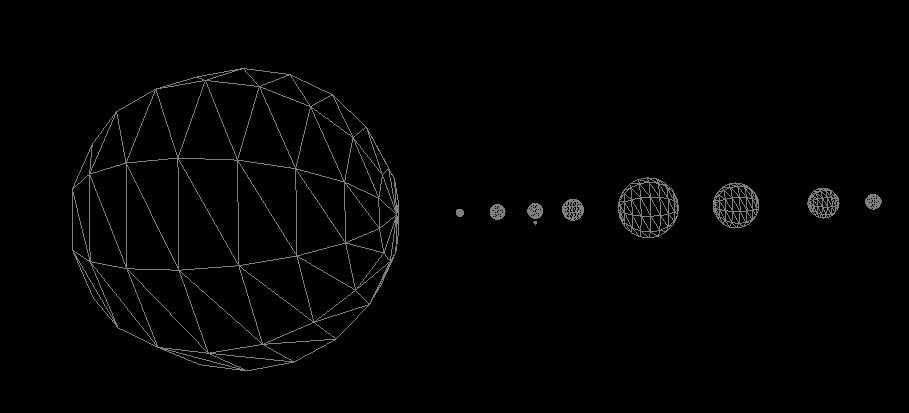
\includegraphics[width=12cm,height=6cm]{capa}
\end{figure}
\newpage

\begin{abstract}
A \textbf{Computação Gráfica}, uma das muitas áreas da informática, que assume um papel fulcral em interações homem-máquina e na visualização de dados. o seu espectro de aplicações varia desde geração de imagens até a simulação do mundo real. \par
	O presente relatório refere-se às diferentes fases de entrega da componente prática da Unidade Curricular de \textbf{Computação Gráfica} enquadrada no curso de \textit{Ciências da Computação} da \textit{Universidade do Minho}. 
\end{abstract}
\newpage

%-------------------------------------------------
% 		METER A QUOTE AQUI
%-------------------------------------------------

\tableofcontents{}
\newpage

%-------------------------------------------------
%		Introducao
%-------------------------------------------------


\section{Introdução}
Na primeira fase, foram desenvolvidas duas aplicações. Um \textbf{Gerador} de modelos, que aceite argumentos a partir do terminal, com a função de gerar os pontos de uma primitiva gráfica desejada pelo utilizador, imprimindo estes para um ficheiro. E a última, um \textbf{Motor} que interpreta os pontos gerados anteriormente de acordo com um ficheiro de configuração dado. 
Com base nos tópicos enunciados e ferramentas exploradas nas aulas implementamos o \textbf{Gerador} e o \textbf{Motor} na linguagem \textbf{C++}. Em particular esta última faz uso de biblioteca \textbf{TinyXML2} para que a leitura dos documentos que lhe são dados com input seja feita de forma simples e consistente. E por fim,  utilizamos a API fornecida pelo \textbf{OpenGl} para dar vida aos nossos modelos.\\
Na segunda, adicionamos features ao parser de ficheiros de configuração de \textbf{scenes}, nomeadamente, o reconhecimento de \textbf{scenes} dispostas hierarquicamente usando transformações geométricas (translações, rotações e de escala).
\newpage

\section{Primeira Fase}

\subsection{Gerador}
O nosso \textbf{Gerador} é um pequeno programa em \textbf{C++}, cuja implementação é disponibilizada em anexo, que depois de compilado, o correspondente executável escreve para um ficheiro (um por linha) os vértices da primitiva gráfica desejada  como iremos ilustrar nas seguintes secções.


\subsubsection{Caixa}
Para geração desta primitiva o utilizador deverá invocar a aplicação a com o nome do executável seguido dos comprimentos dos lados de um paraleloipipedo no eixos com X’s, Y’s e Z’s respetivamente e por fim o nome do ficheiro destino. A sintaxe é demonstrada no exemplo abaixo:

\begin{commandline}
    \begin{verbatim}
        $ g++ -o gerador gen.cpp
        $ ./gerador caixa 3 4 5 osmeusvertices
        $ ls
        $ gen.cpp            gerador            osmeusvertices.txt
    \end{verbatim}
\end{commandline}

\begin{figure}[H]
	\centering
	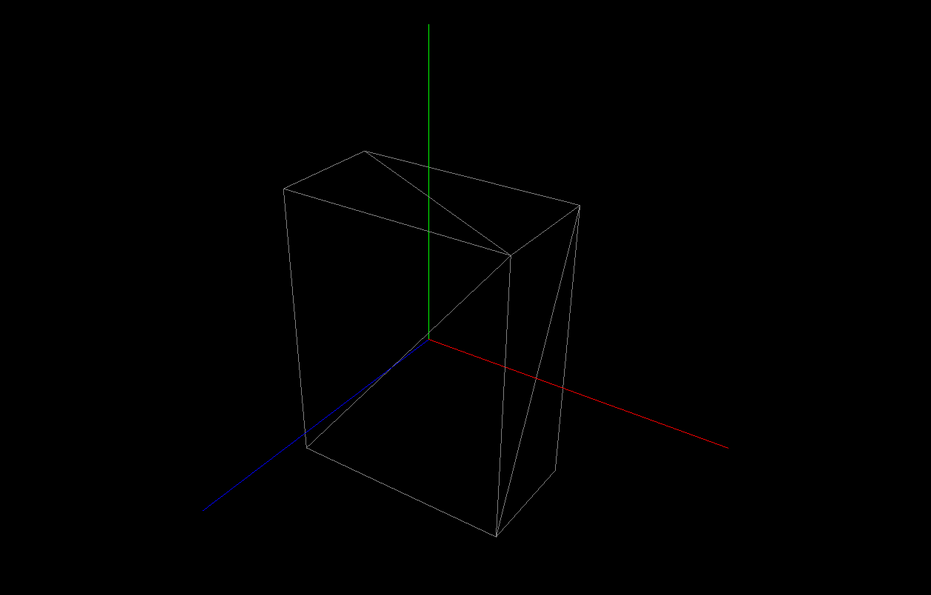
\includegraphics[width=4cm,height=4cm]{caixa}
	\caption{Caixa}
\end{figure}

\begin{warn}[Notice:]
Todas as faces são desenhadas com dois triângulos apontados para o exterior pela norma da mão direita mencionada nas aulas. Um zoom excessivo, ou a escolha de dimensões superiores à distância da câmara à origem(onde este é centrado)  pode levar ao aparente desaparecimento do modelo.
\end{warn}

\subsubsection{Cone}
O \textbf{Cone} recebe como argumentos o raio da base, a sua altura, o número de slices e stacks. \\
A construção deste começa por fixar um uma \textit{slice} calculando os vértices da base correspondente, de seguida todas as \textit{stacks} relativas, sendo o última stack - a do bico - um caso especial. \\
O algoritmo usa noções como semelhança de triângulos para cálculo dos sucessivos raios das circuferências formadas pelas \textit{stacks}.\\

\begin{info}
	Apresentamos o significado das variáveis usadas no programa que gera os pontos do \textbf{Cone}: 
	\begin{itemize}
		\item[] \textit{stkd} - diferença entre stacks consecutivas
		\item[] \textit{slcd} - diferença entre slices consecutivas
		\item[] \textit{raiod} - diferença entre o raio de duas stacks consecutivas
		\item[] \textit{stk} - stack atual 
		\item[] \textit{slc} - slice atual
		\item[] \textit{nslc} - próxima slice
		\item[] \textit{nstk} - próxima stack
		\item[] \textit{nr} - próximo raio
		\item[] \textit{r} - raio atual
	\end{itemize}
\end{info}

\begin{figure}[H]
	\centering
	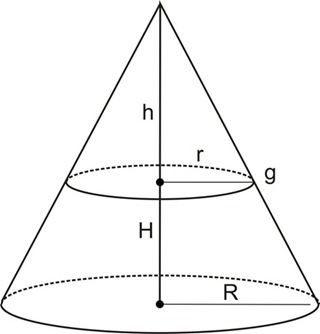
\includegraphics[width=4cm,height=4cm]{conesemelhante}
	\caption{Semelhança de triângulos num cone}
\end{figure}

Apresentamos algumas imagens que ilustram a criação do cone. \\

\begin{figure}[H]
	\centering
	\subfloat[2 stacks]{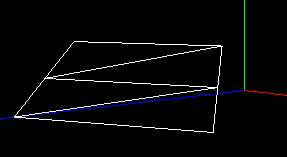
\includegraphics[width=3cm,height=3cm]{2stk}}
	\hspace{2cm}
	\subfloat[4 stacks]{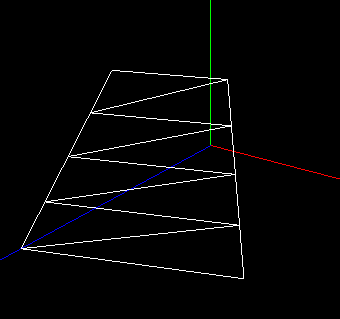
\includegraphics[width=3cm,height=3cm]{4stk}}
	\caption{Progessão das stacks do cone}
\end{figure}

\begin{figure}[H]
	\centering
	\subfloat[1 slice]{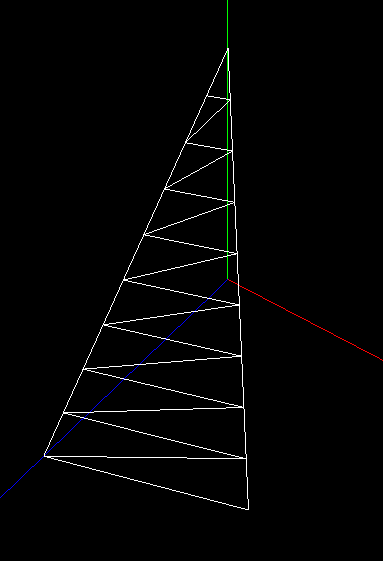
\includegraphics[width=3cm,height=3cm]{1slc}}
	\hspace{2cm}
	\subfloat[2 slices]{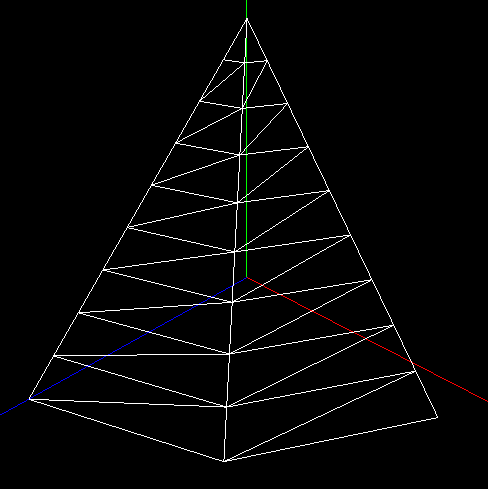
\includegraphics[width=3cm,height=3cm]{2slc}}
	\caption{Progessão das slices do cone}
\end{figure}

Finalmente obtemos:

\begin{figure}[H]
	\centering
	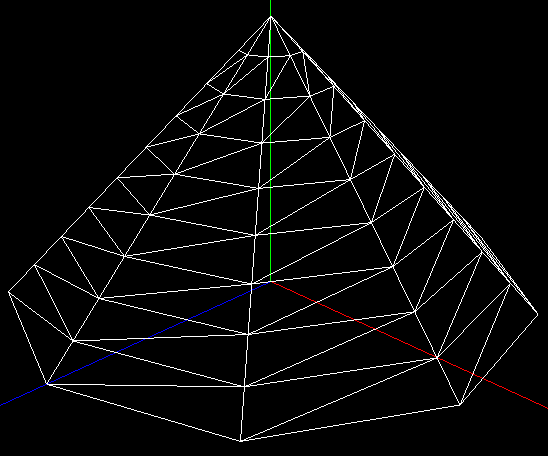
\includegraphics[width=4cm,height=4cm]{cone}
	\caption{Cone}
\end{figure}

\subsubsection{Esfera}
A \textbf{Esfera} recebe como argumentos o seu raio, o número de slices e stacks.
A sua construção usa coordenadas esféricas usando o raio dado como argumentos e manipulando 2 ângulos \textit{Alfa} e \textit{Beta}. \textit{Alfa} é dado por: \\
\[ alfa = \frac{2\times \Pi}{slices} \]
Este nos programas é usado juntamente com o raio para calcular os pontos de \textit{slices} consecutivas. De seguida \textit{beta} é dado por:\\
\[ beta = \frac{\Pi \div 2}{stacks}\] \\
Este desenpenha uma função igual ao anterior considerando \textit{stacks}.\\


\begin{figure}[H]
	\centering
	\subfloat[4 stacks]{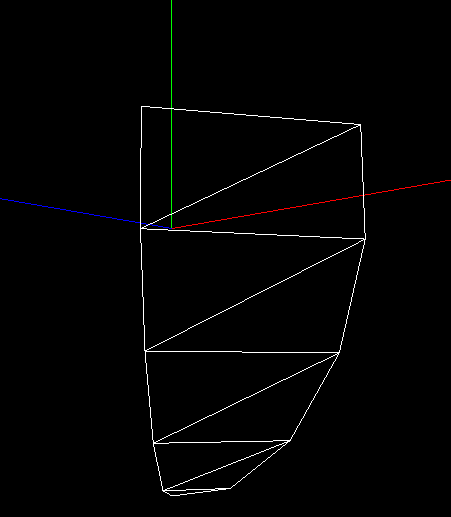
\includegraphics[width=3cm,height=3cm]{4estk}}
	\hspace{2cm}
	\subfloat[8 stacks]{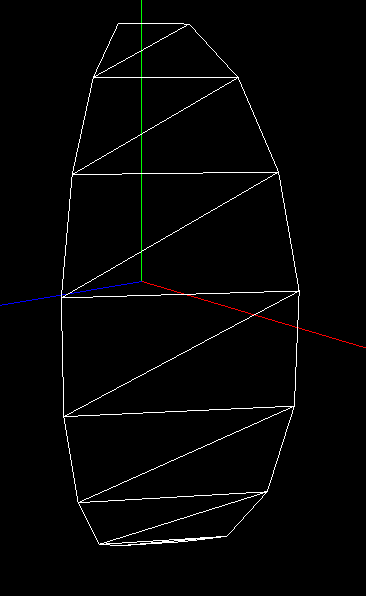
\includegraphics[width=3cm,height=3cm]{8estk}}
	\caption{Progessão das stacks da esfera}
\end{figure}

\begin{figure}[H]
	\centering
	\subfloat[1 slice]{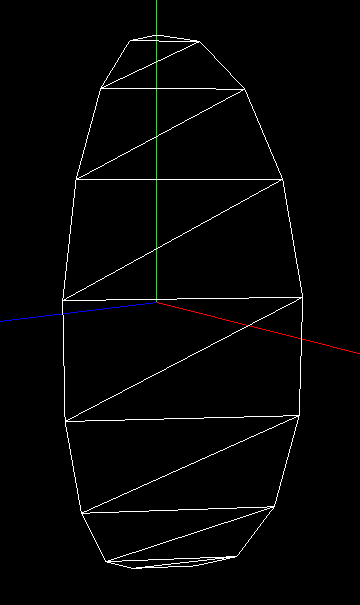
\includegraphics[width=3cm,height=3cm]{1eslc}}
	\hspace{2cm}
	\subfloat[2 slices]{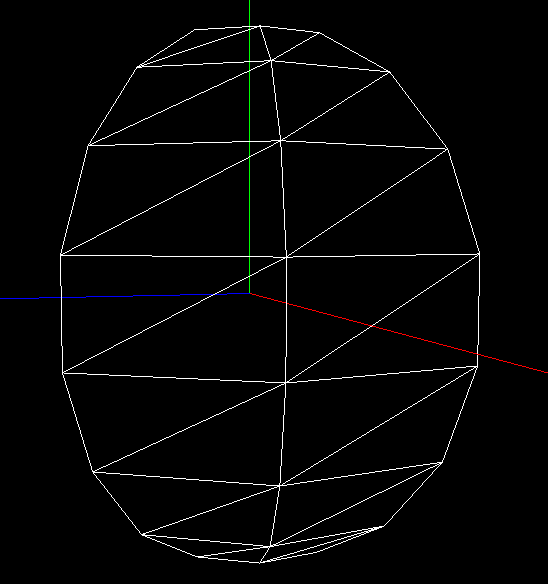
\includegraphics[width=3cm,height=3cm]{2eslc}}
	\caption{Progessão das slices da esfera}
\end{figure}

\begin{figure}[H]
	\centering
	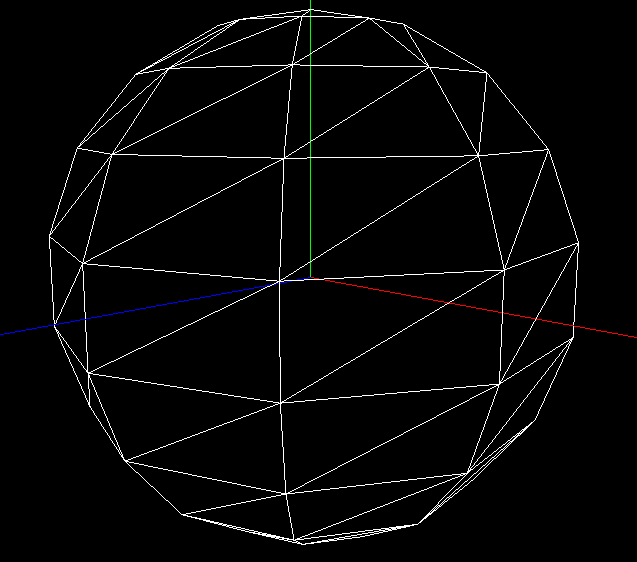
\includegraphics[width=4cm,height=4cm]{esfera}
	\caption{Esfera}
\end{figure}

\subsubsection{Plano}
O requisito estabelecido no guião do trabalho veio em muito simplificar a representação do plano XZ ao ponto de para a sua computação seja apenas necessário um único argumento que representa o tamanho da porção visível desejada.  

\begin{commandline}
    \begin{verbatim}
        $ g++ -o gerador gen.cpp
        $ ./gerador plano 5 pontos
        $ ls
        $ gen.cpp            gerador            pontos.txt
    \end{verbatim}
\end{commandline}

\begin{figure}[H]
	\centering
	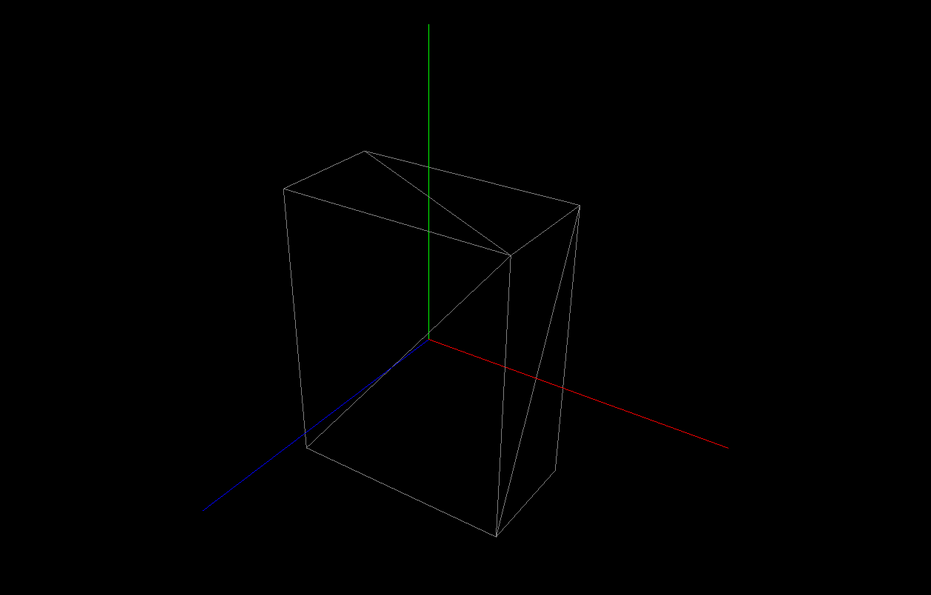
\includegraphics[width=4cm,height=4cm]{caixa}
	\caption{Caixa}
\end{figure}

\begin{warn}[Notice:]
Os planos são infinitos a referência ao tamanho é feita apenas para facilitar a observação do mesmo.
São desenhados 4 triângulos, em vez de dois, para que esta primitiva seja visível de todas as perspectivas.
\end{warn}

\newpage
\subsection{Motor}
O motor é a parte do nosso trabalho que faz o linking de todas as outras partes que foram realizadas. O motor, lê um ficheiro xml (conf.xml). Este ficheiro contém uma estrutura bastante simples, dividida em scenes.

% Contents do ficheiro conf.xml
\begin{file}[conf.xml]
	\begin{lstlisting}[language=XML]
	<scene>
		<model file="esfera.txt" />
		<model file="cone.txt" />
		<model file="caixa.txt" />
	</scene>
	\end{lstlisting}
	\end{file}

Cada ficheiro que está referenciado nas tags \textbf{<model>} é um ficheiro de texto criado pelo nosso gerador e contém todos os pontos das figuras que queremos representar.
Como o motor lê os ficheiros de pontos a partir dum ficheiro \textbf{XML} utilizamos um parser xml para \textbf{C++} chamado \textbf{tinyxml-2}.

\begin{file}[main.cpp]
	\begin{lstlisting}[language=C++]
...
tinyxml2::XMLDocument doc;

doc.LoadFile("./conf.xml");

tinyxml2::XMLNode *scene = doc.FirstChild();
		
tinyxml2::XMLElement* model;

while(scene) {
	for(model = scene->FirstChildElement();
	model != NULL; 
	model = model->NextSiblingElement()) {
		const char * file;
		file = model->Attribute("file");
		guardaPontos(file);
	}
	scene = scene->NextSiblingElement();
}
...

	\end{lstlisting}
\end{file}

Com este snippet de código, criamos um objeto do tipo XMLDocument. De seguida, com a função \textbf{LoadFile}, abrimos o ficheiro de configuração \textbf{conf.xml}, e começamos a manipular o seu conteúdo.
Criamos um objeto do tipo \textbf{XMLNode} e associamos-lhe a primeira \textbf{tag} do ficheiro conf.xml que é a raiz da estrutura do nosso ficheiro.
No ciclo while, percorremos todos o ChildElements de scene, que são as tags que guardam os nossos ficheiros das figuras.
Cada ficheiro de figura tirado dos \textbf{models} é passado à função \textbf{guardaPontos}, que será explicada de seguida.

\begin{file}[main.cpp]
	\begin{lstlisting}[language=C++]
...
struct Pontos {
    float a;
    float b;
    float c;
};

std::vector<Pontos> pontos;

void guardaPontos(std::string ficheiro) {
	std::ifstream file;
	std::string s = "./";
	s.append(ficheiro.c_str());
	file.open(s.c_str());
	float a,b,c;
	while(file >> a >> b >> c) {
		Pontos aux;
		aux.a = a;
		aux.b = b;
		aux.c = c;
		pontos.push_back(aux);
	}
}
...
	\end{lstlisting}
\end{file}

Criamos uma estrutura \textbf{Pontos} que tem como campos 3 \textit{floats}, que servem para registar as coordenadas destes. De seguida usamos um vector que utiliza a estrutura enunciada para os guardar.
À função \textbf{guardaPontos} são passados nomes de ficheiros. A função abre os ficheiros e lê pontos linha a linha, guardando cada coordenada \textit{x, y e z} num \textbf{Ponto} e de seguida inserindo-o no vector.

\begin{info} % Information block
	A instrução:
	\begin{lstlisting}[language=C++]
		file >> a >> b >> c
	\end{lstlisting}
	associa a cada uma das variaveis \textit{a, b} e \textit{c}, as coordenadas da linha que está a ser lida em cada iteração do ciclo.
\end{info}

Por ultimo temos a função \textbf{printPontos}:

\begin{file}[main.cpp]
	\begin{lstlisting}[language=C++]
...
void printPontos(std::vector<Pontos> pontos) {
  for(int i = 0; i < pontos.size(); i++) {
		glVertex3f(pontos[i].a,
			pontos[i].b, 
			pontos[i].c);
	}
}
...
	\end{lstlisting}
\end{file}

Esta função é chamada na \text{renderScene} e geras todos os pontos percorrendo o vector.

\newpage

\section{Segunda Fase}
Após ponderarmos o enunciado, o grupo(e não o césar), decidiu implementar uma classe, em \textbf{C++}, inspirada numa estrutura de dados largamente conhecida na área, denominada por \textbf{Scene Graph}.\\
A origens desta estrutura de dados remonta aos primórdios dos primeiros jogos de vídeo sobre simulação de voo mas actualmente é vulgarmente incluída qualquer aplicação que lide com \textbf{Graphic Rendering}.\\
Esta estrutura de dados foi revolucionária pelo facto de reduzir drasticamente a memória necessária em cálculos sistemáticos sobre o mundo que está a tentar representar. Os cálculos passaram a ser feitos \textbf{in place} na estrutura dispensando na totalidade a necessidade de memória auxiliar. 

\subsection{A classe Scene Graph}
Apesar de disponibilizarmos a implementação em anexo iremos contemplar alguns pormenores neste capítulo.\\
Face a como os ficheiros \textbf{XML} são organizados via uma \textit{árvore} - \textit{DOM Tree} - implementamos uma classe que usa os princípios de essa mesma estrutura para guardar os dados de tudo o que é exposto na cena.\\
Por exemplo se quiséssemos desenhar um cavalo e o seu cavaleiro, não de maneira independente, mas como se o cavalo fosse uma extensão do seu cavaleiro. O \textbf{Scene Graph} correspondente teria no nodo \textbf{Cavalo} “pendurado” no nodo \textbf{Cavaleiro}.\\
Cada nodo, é um \textbf{Group} e nele guardamos as transformações geométricas que a ela lhe dizem respeito assim como um vector de pontos do \textbf{model} que queremos desenhar, e por fim, um array de outros \textbf{Scene Graphs} que representam o próximo nível de descendentes.\\

\begin{file}[main.cpp]
    \begin{lstlisting}[language=C++]

class SceneGraph {
    
    array<float, 3> scale;
    array<float, 3> trans;
    array<float, 4> rot;
    vector<vector<Ponto>> modelos;
    vector<SceneGraph> filhos;

}

    \end{lstlisting}
\end{file}

Estamos então perante a definição de uma árvore de \textbf{Scene Graphs}. Para facilitar a visualização deste conceito dispomos o seguinte exemplo.

\begin{figure}[H]
    \centering
    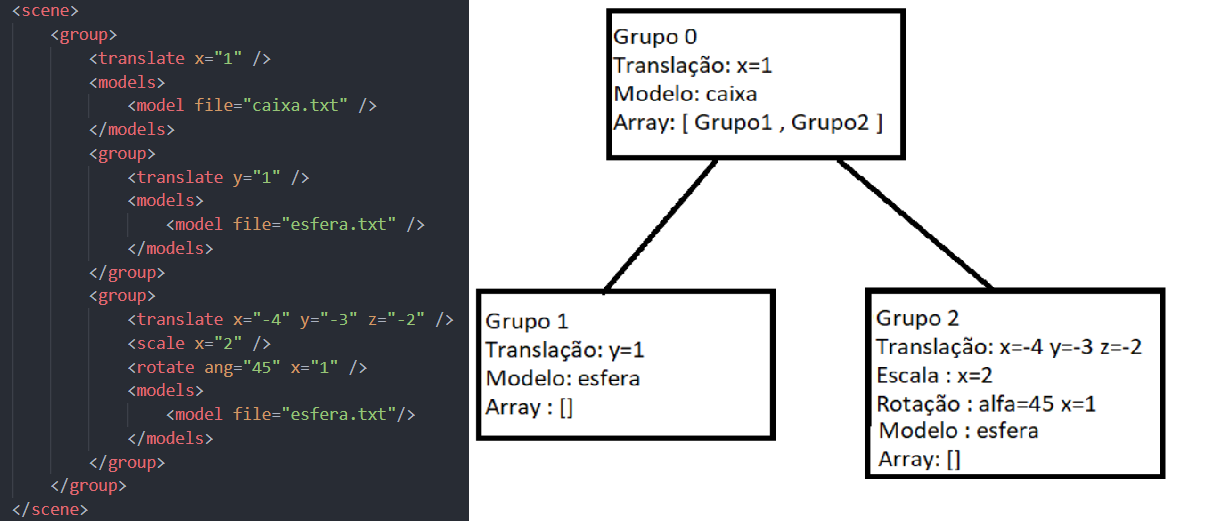
\includegraphics[width=16cm,height=6cm]{exemplo}
\end{figure}

\begin{info}
    \begin{itemize}
        \item Todos os nodos filhos herdam as transformações dos pais.
        \item Cada nodo pode ter um qualquer número de filhos, mas apenas um pai, i.e., não existe herança múltipla.
        \item Da travessia desde a raiz, até a uma folha, resultam todas as dependências que um certo objecto tem na \textbf{scene} em questão.
    \end{itemize}
\end{info}

Fixada a estrutura e comportamento do classe. Basta, agora, expor o algoritmo de travessia que é efectuada quando a nossa modesta aplicação lê um ficheiro de configuração. O resto da \textbf{API} é disponibilizada em anexo.

\begin{file}[main.cpp]
    \begin{lstlisting}[language=C++]
void SceneGraph::draw() const {

	glPushMatrix();

	glScalef(scale[0], scale[1], scale[2]);
	glRotatef(rot[0], rot[1], rot[2], rot[3]);
	glTranslatef(trans[0], trans[1], trans[2]);
	
	glBegin(GL_TRIANGLES);
	
	for( vector<Pontos> const &pnts : 
		this->modelos ) {	
		for( Pontos const &p : pnts ) {
        		glVertex3f(p.a, p.b, p.c);
    		}
	}

	glEnd();

	for( SceneGraph const &tmp : 
		this->filhos ) {
		tmp.draw();
	}

	glPopMatrix();

}   
    \end{lstlisting}
\end{file}

\begin{info}
Com base nos conteúdos abordados nas aulas teóricas decidimos adotar a convenção de ordenar as transformações geométricas \textbf{glRotatef()},\textbf{glTranslatef()} e \textbf{glSclasef()} pela sequência exposta no código acima.
\end{info}

\newpage
\subsection{Motor}
De maneira semelhante à primeira fase, o motor continua a fazer leituras de um ficheiro xml (conf.xml). Por outro lado, este ficheiro apresenta uma complexidade superior ao anterior, contendo groups, models e ainda tags de translação (\textbf{<translate>}), rotação (\textbf{<rotate>}) e mudança de escala (\textbf{<scale>}).

% Contents do ficheiro conf.xml
\begin{file}[conf.xml]
	\begin{lstlisting}[language=XML]
<scene>
    <group>
        <translate x="1" />
        <models>
            <model file="caixa.txt" />
        </models>
        <group>
            <translate y="1" />
            <models>
                <model file="esfera.txt" />
            </models>
        </group>
        <group>
            <translate x="-4" y="-3" z="-2" />
            <scale x="2" />
            <rotate ang="45" x="1" />
            <models>
                <model file="esfera.txt"/>
            </models>
        </group>
    </group>
</scene>
	\end{lstlisting}
	\end{file}

Cada ficheiro que está referenciado nas tags \textbf{<model>} é um ficheiro de texto criado pelo nosso gerador e contém todos os pontos das figuras que queremos representar.
Como o motor lê os ficheiros de pontos a partir dum ficheiro \textbf{XML} utilizamos um parser xml para \textbf{C++} chamado \textbf{tinyxml-2}.

\begin{file}[main.cpp]
	\begin{lstlisting}[language=C++]
...
tinyxml2::XMLDocument doc;
//new file
doc.LoadFile("./conf.xml");
tinyxml2::XMLNode *scene = doc.FirstChild();
if (scene == nullptr) perror("Erro de Leitura.\n");

s_gg = doGroup(scene->FirstChildElement("group"));
...
	\end{lstlisting}
\end{file}

Com este snippet de código, criamos um objeto do tipo XMLDocument. De seguida, com a função \textbf{LoadFile}, abrimos o ficheiro de configuração \textbf{conf.xml}, Criamos um objeto do tipo \textbf{XMLNode} e associamos-lhe a primeira \textbf{tag} do ficheiro conf.xml que é a raiz da estrutura do nosso ficheiro.
Através da função doGroup, começamos a manipular o seu conteúdo.

\begin{file}[engine.cpp]
	\begin{lstlisting}[language=C++]
SceneGraph doGroup(tinyxml2::XMLElement* group) {
    SceneGraph s_g;
    tinyxml2::XMLElement* novo = 
	group->FirstChildElement();
    for(novo; novo != NULL; 
	novo = novo->NextSiblingElement()) {
        //printf("%s\n", novo->Name());
        if(!strcmp(novo->Name(), "group")) {
            s_g.addFilho(doGroup(novo));
        } else if(!strcmp(novo->Name(), "models")) {
            s_g.setModelo(doModels(novo));
        } else if(!strcmp(novo->Name(), 
		"translate")) {
            s_g.setTrans(doTranslate(novo));
        } else if(!strcmp(novo->Name(), "rotate")) {
            s_g.setRot(doRotate(novo));
        } else if(!strcmp(novo->Name(), "scale")) {
            s_g.setScale(doScale(novo));
        } else {
            perror("Formato XML Incorreto.\n");
        }
    }
return s_g;
}
	\end{lstlisting}
\end{file}

No ciclo \textit{for}, percorremos todos o ChildElements da group, que são as tags que guardam os nossos ficheiros das figuras.
Dentro de cada tag \textbf{group} pode haver outra tag \textbf{group}, ativando a recursão da função doGroup. Mas, há outras tags que podem aparecer, tais como \textbf{models} \textbf{<translate>}, \textbf{<rotate>} e \textbf{<scale>}.
Caso a tag lida seja \textbf{<translate>}, a função doGroup evoca a função doTranslate:

\begin{file}[engine.cpp]
	\begin{lstlisting}[language=C++]
array<float,3> doTranslate(
	tinyxml2::XMLElement* translate) {

    array<float, 3> trans;
    
    const char * x;
    const char * y;
    const char * z;
    x = translate->Attribute("x");
    y = translate->Attribute("y");
    z = translate->Attribute("z");
    
    x == nullptr ? trans[0] = 0 : trans[0] = atof(x);
    y == nullptr ? trans[1] = 0 : trans[1] = atof(y);
    z == nullptr ? trans[2] = 0 : trans[2] = atof(z);
    
    return trans;
}
	\end{lstlisting}
\end{file}

Caso a tag lida seja \textbf{<rotate>}, a função doGroup evoca a função doRotate:

\begin{file}[engine.cpp]
	\begin{lstlisting}[language=C++]
array<float,4> doRotate(tinyxml2::XMLElement* rotate) {

    array<float,4> rot;

    const char * x;
    const char * y;
    const char * z;
    const char * ang;
    x = rotate->Attribute("x");
    y = rotate->Attribute("y");
    z = rotate->Attribute("z");
    ang = rotate->Attribute("angle");

    ang == nullptr ? rot[0] = 0 : rot[0] = atoi(ang);
    x == nullptr ? rot[1] = 0 : rot[1] = atof(x);
    y == nullptr ? rot[2] = 0 : rot[2] = atof(y);
    z == nullptr ? rot[3] = 0 : rot[3] = atof(z);

    return rot;	
}
	\end{lstlisting}
\end{file}

Caso a tag lida seja \textbf{<scale>}, a função doGroup evoca a função doScale:

\begin{file}[engine.cpp]
	\begin{lstlisting}[language=C++]
array<float,3> doScale(tinyxml2::XMLElement* scale) {

    array<float,3> sca;
    
    const char * x;
    const char * y;
    const char * z;
    
    x = scale->Attribute("x");
    y = scale->Attribute("y");
    z = scale->Attribute("z");
    
    x == nullptr ? sca[0] = 1 : sca[0] = atof(x);
    y == nullptr ? sca[1] = 1 : sca[1] = atof(y);
    z == nullptr ? sca[2] = 1 : sca[2] = atof(z);
    
    return sca;
}
	\end{lstlisting}
\end{file}

Qualquer uma destas 3 funções, retorna um array com os argumentos que serão passados às funções Glut que executarão as transformações: a função doTranslate, retorna um array com 3 argumentos para a função \textbf{glTranslate}, a função doRotate, retorna um array com 4 argumentos para a função \textbf{glRotate} e a função doScale, retorna um array com 3 argumentos para a função \textbf{glScale}.

\par Por outro lado, ainda pode aparecer uma tag \textbf{<models>}, ou seja é chamada a função doModels que significa que, dentro dessas tags, vai haver uma tag \textbf{<model file= "nome do ficheiro.txt">}, ficheiro este que tem todos os pontos gerados pelo gerador. 

\begin{file}[engine.cpp]
	\begin{lstlisting}[language=C++]
std::vector<std::vector<Pontos>> 
	doModels(tinyxml2::XMLElement* models) {
    std::vector<std::vector<Pontos>> pPontos;
    tinyxml2::XMLElement* novo = 
	models->FirstChildElement();
    for(novo; novo != NULL; 
	novo = novo->NextSiblingElement()) {
        const char * file;
        file = novo->Attribute("file");
        pPontos.push_back(guardaPontos(file));
    }
    return pPontos;
}
	\end{lstlisting}
\end{file}
	
A função doModels chama a função \textbf{guardaPontos} que, usando a estrutura \textbf{Pontos}, regista as coordenadas de cada ponto presente no ficheiro. A estrutura tem campos 3 \textit{floats}, que servem para guardar as coordenadas dos pontos. De seguida usamos um vector que utiliza a estrutura enunciada para os guardar.
A função abre os ficheiros e lê pontos linha a linha, guardando cada coordenada \textit{x, y e z} num \textbf{Ponto} e de seguida inserindo-o no vector.

\begin{file}[engine.cpp]
	\begin{lstlisting}[language=C++]
...
struct Pontos {
    float a;
    float b;
    float c;
};

std::vector<Pontos> pontos;

void guardaPontos(std::string ficheiro) {
	std::ifstream file;
	std::string s = "./";
	s.append(ficheiro.c_str());
	file.open(s.c_str());
	float a,b,c;
	while(file >> a >> b >> c) {
		Pontos aux;
		aux.a = a;
		aux.b = b;
		aux.c = c;
		pontos.push_back(aux);
	}
}
...
	\end{lstlisting}
\end{file}

Este array de pontos que a guardaPontos retorna, preenche o array pPontos instanciado na doModels, que por sua vez é retornado por esta função. Na função doGroup, uma SceneGraph é passada como objeto aos Setters definidos na estrutura SceneGraph, que chamam as funções acima faladas que, retornandos os arrays de argumentos e os pontos das figuras, fazem uma atualização da estrutura, que na \textbf{main.cpp} é passada à renderScene.
\newpage

\section{Conclusão}
Também nos ajudou a possuir mais discernimento sobre a geometria e cálculos matemáticos por detrás de todo um esquema geométrico em 3 dimensões.\\
Durante a realização dos geradores conseguimos perceber que a propagação dos erros nos cálculos dos ângulos pode ter impacto na apresentação das figuras geométricas.\\
Apresentou-nos também mais uma oportunidade de aprender e melhorar as nossas capacidades de programação em C++, no uso de LaTex e de ficheiros XML.\\
Todas as aptidões aqui aprendidas e/ou desenvolvidas, não só a nível escolar mas como a nível de cooperação e  de trabalho de equipa. vão-nos permitir uma melhor realização de projetos futuros.\\
Está secção poderá ser modificada ao longo das fases de entrega.\\

\newpage


\appendix

\section{Código do Gerador}

\lstinputlisting[language=C++]{gen.cpp}

\newpage

\section{Código do Motor}

\lstinputlisting[language=C++]{./Deps/engine.cpp}

\newpage

\section{Código do ficheiro SceneGraph.h}

\lstinputlisting[language=C++]{./Deps/sg.h}

\newpage

\section{Codigo do SceneGraph.cpp}

\lstinputlisting[language=C++]{./Deps/sg.cpp}

\newpage 

\section{Código da Main}

\lstinputlisting[language=C++]{main.cpp}

\end{document}
